%\section{Cele i założenia projektowe}

%\newpage

\section{Wstęp teoretyczny}

\subsection{Sieci Bayesowskie}

\textbf{Definicja Sieci Bayesowskiej}
\newline
\textit{Siecią Bayesa nazywamy skierowany graf acykliczny o wierzchołkach reprezentujących zmienne losowe i łukach określających zależności. Istnienie łuku pomiędzy dwoma wierzchołkami oznacza istnienie bezpośredniej zależności przyczynowo skutkowej pomiędzy odpowiadającymi im zmiennymi. Siła tej zależności określona jest przez tablice prawdopodobieństw warunkowych.}\newline

Inaczej mówiąc, sieć Bayesowska to acykliczny (nie zawierający cykli) graf skierowany, w którym:
\begin{itemize}
\item Węzły reprezentują zmienne losowe (np. temperaturę jakiegoś źródła, stan pacjenta, cechę obiektu itp.)
\item Łuki (skierowane) reprezentują zależnośd typu „zmienna X ma bezpośredni wpływ na zmienna Y”,
\item Każdy węzeł X ma stowarzyszona z nim tablice prawdopodobieostw warunkowych określających wpływ wywierany na X przez jego poprzedników (rodziców) w grafie.
\item Zmienne reprezentowane przez węzły przyjmują wartości dyskretne.
\end{itemize}

\begin{figure}[h!]
	\centering
	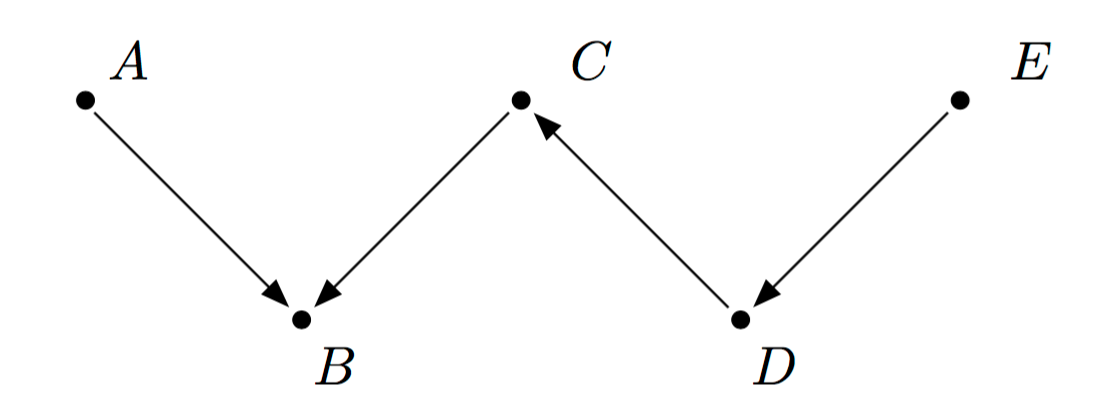
\includegraphics[height=3cm]{bayes1.png}
	\label{bayes1}
	\caption{Przykładowa sieć Bayesowska}
\end{figure}

Na rysunku został przedstawiony przykład nieskomplikowanej sieci Bayesowskiej. Na podstawie zaprezentowanego na rysunku grafu przedstawiającego sieć można wyciągnąć następujące wnioski:
\begin{itemize}
\item Para zmiennych A oraz B jest od siebie bezpośrednio zależna.
\item Para zmiennych B oraz C jest od siebie bezpośrednio zależna.
\item Zmienna reprezentowana przez wierzchołek B jest jednocześnie zależna od A oraz C.
\item Zmienne A oraz C pozostają brzegowo niezależne do momentu ustalenia wartości B (własność tą można również określić mówiąc, że zmienne A i C są d-połączone).
\item Zmienne E oraz C są zależne pośrednio.
\item Zmienna D d-separuje zmienne C i E.
\item Zmienne C i D d-separują parę zmiennych B, E.
\end{itemize}

\textbf{Orientacja łuków jest konieczna do określenia zależności nieprzechodnich.} Na przytoczonym przykładzie można zaobserwować, że pomimo faktu przemienności własności zależności orientacja krawędzi wnosi istotną informację o rozkładzie.\newline

Sieć Bayesowska pozwala na wyznaczenie rozkładu prawdopodobieństwa zmiennych. Jeżeli przez \(\Pi\)(Xi) oznaczymy zbiór rodziców danego wierzchołka w grafie, to rozkład prawdopodobieństwa zmiennych danej sieci opisuje się równaniem:
$$ P(X_{1}, X_{2}, ... , X_{n}) = \prod _{i=1}^{n}P(X_{i} | \Pi (X_{i})) $$

Co dla przedstawionego powyżej przykładu wynosi:
$$ P(A,B,C,D,E) = P(A)P(B|A,C)P(C|D)P(D|E)P(E) $$ 

Dzięki powyższemu równaniu równania możliwe jest określenie prawdopodobieństwa wystąpienia określonego wartościowania wszystkich zmiennych, znając jedynie lokalne prawdopodobieństwa warunkowe. Określając wartości tzw. \textit{przyczyn podstawowych}, czyli węzłów grafu nie posiadających rodziców (zmienne A, E w podanym przykładzie), można określić wartości oczekiwane innych atrybutów. Wszystkie pozostałe zmienne zależą bowiem pośrednio lub bezpośrednio od tego zbioru.

Istotą działania sieci Bayesowskich jest propagacja informacji o rozkładzie prawdopodobieństwa. 
W praktyce jednak \textbf{sieci Bayesowskie używane są do ekstrakcji informacji o rozkładach nieznanych, o których wiadomości możemy czerpać tylko z dostępnych wyników prób z eksperymentów statystycznych.} Sieci te nie są zatem używane do opisywania dokładnych rozkładów.

Próby z eksperymentów statystycznych (zestawy danych uczących) mogą mieć bardzo duże rozmiary, a ekstrakcja zawartych w nich w nich informacji może być zadaniem bardzo złożonym obliczeniowo. Proces uczenia sieci może być zatem postrzegany jako statystyczna kompresja informacji o rozkładzie do zwartej i jednocześnie bardziej przydatnej do wnioskowania bayesowskiego postaci.

Konstruowanie sieci Bayesowskiej składa się z następujących kroków:
\begin{itemize}
\item zdefiniowanie zmiennych,
\item zdefiniowanie połączeń pomiędzy zmiennymi,
\item określenie prawdopodobieństw warunkowych \textit{a priori}
\item wprowadzenie danych do sieci,
\item uaktualnienie sieci,
\item wyznaczenie prawdopodobieństw \textit{a posteriori}
\end{itemize}

Uczenie sieci jest uczeniem bez nadzoru i bez wstępnej wiedzy eksperckiej, a co za tym idzie zakłada się, że na wstępie (bez znajomości próby statystycznej) wszystkie dozwolone struktury sieci są jednakowo prawdopodobne, a przy ustalonej strukturze grafu wszystkie możliwe poprawne zbiory tablic prawdopodobieństw warunkowych są jednakowo prawdopodobne.

\subsubsection{Algorytm Chow-Liu}
Algorytm Chow-Liu stanowi klasyczny algorytm odtwarzający kształt zależności w próbie. Algorytm nie buduje sieci Bayesowskiej, a jedynie niezorientowane drzewo zależności. Jeżeli sieć Bayesa danego rozkładu ma postać drzewa, to algorytm Chow-Liu poprawnie odtworzy jego kształt. Algorytm Chow-Liu nie sprawdza, czy rozkład zmiennych zadanej próby D spełnia powyższy warunek. Jeśli struktura zależności między zmiennymi w próbie nie jest drzewem, to algorytm znajduje najlepszą strukturę drzewiastą, która opisuje postać zależności. Należy jednak pamiętać, że w skrajnie niekorzystnych wypadkach informacja zwrócona przez algorytm może być błędna.\newline

\textbf{Przebieg algorytmu:}\newline
\textbf{Krok 1:} Niech G oznacza graf pełny o zbiorze wierzchołków tożsamym ze zbiorem atrybutów próby D. Wówczas niech T będzie nieskierowaną strukturą drzewiastą uzyskaną w wyniku zastosowania dowolnego algorytmu znajdowania minimalnego drzewa rozpinającego (MST) w grafie G z funkcją wagową określającą stopień zależności między zmiennymi.\newline
\textbf{Krok 2:} W drzewie T należy obrać kierunki w sposób dowolny, uzyskując wynikową strukturę sieci Bayesa BS.\newline

W pierwszym kroku możliwe jest wykorzystanie odległości Kullback-Leiblera jako funkcji wagowej:
$$ DEP(X_{i}, X_{j}) = \sum_{x_{i}, x_{j}}^{ }  P(x_{i}, x_{j}) log \frac{P(x_{i}, x_{j})}{P(x_{i})P(x_{j})} $$

\begin{figure}[h!]
	\centering
	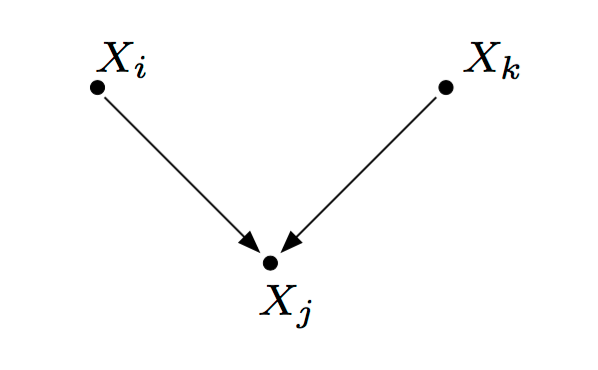
\includegraphics[height=3cm]{bayes2.png}
	\label{bayes2}
	\caption{Dwu rodziców: \(DEP(X_{i},X_{k}) = 0 \wedge DEP(X_{i},X_{k}|X_{j}) > 0\)}
\end{figure}

\begin{figure}[h!]
	\centering
	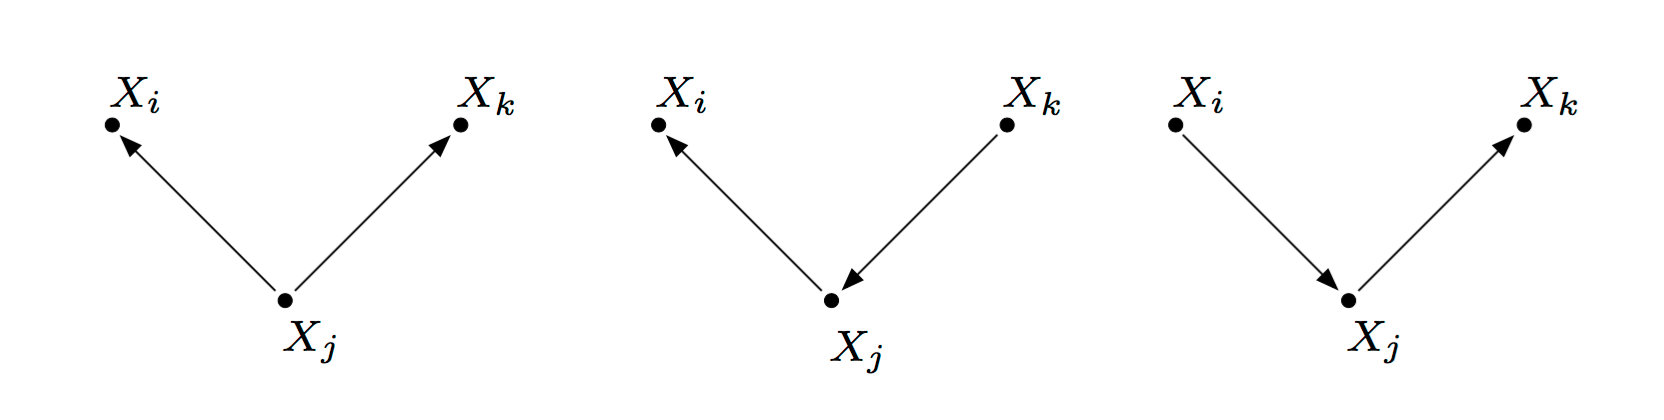
\includegraphics[height=3cm]{bayes3.png}
	\label{bayes3}
	\caption{\( X_{j}\) d-separuje \(X_{i},X_{k}:DEP(X_{i},X_{k})>0 \wedge DEP(X_{i},X_{k}|X_{j})=0\)}
\end{figure}

Gdzie podobnie jak w warunku małe litery \(x_{i}, x_{j}\) oznaczają wartościowania zmiennych \(X_{i}, X_{j} \)a sumowanie przebiega po wszystkich wartościowaniach w próbie D.





\newpage
\newpage

\subsection{Ukryte modele Markowa}

\subsubsection{Wstęp}

Ukryte modele Markowa (ang. \textit{Hidden Markov Model}, w skrócie \textit{HMM}) jest określeniem zaawansowanego modelu statystycznego znajdującego obecnie zastosowanie w wielu dziedzinach inżynierskich, szczególnie tam, gdzie analizowane są zjawiska o charakterze sekwencji losowych zdarzeń jak na przykład mowa czy gesty. Termin ten został wprowadzony i opisany matematycznie w drugiej połowie lat sześćdziesiątych ubiegłego wieku przez Bauma i Petriego, zaś swą nazwę zawdzięcza podstawie matematycznej, na której się opiera - łańcuchowi Markowa, który to określony został przez rosyjskiego matematyka Andrieja Markowa.

\begin{wrapfigure}{R}{0.5\textwidth}
  \centering
  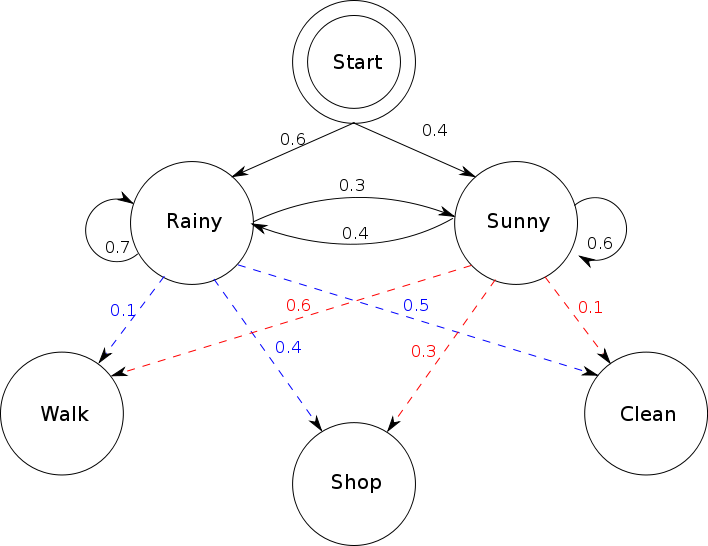
\includegraphics[width=0.5\textwidth]{markov.png}
  \caption{\label{fig:markov}Ogólny wygląd modelu Markowa.}
\end{wrapfigure}

W rozumieniu ogólnym ukryte modele Markowa określają system zdolny z pewnym prawdopodobieństwem przewidzieć jak zachowa się modelowany obiekt w przyszłości, bazując tylko i wyłącznie na jego aktualnym stanie, gdyż nie jest przechowywana historia wyników, jakie osiągał w przeszłości. Cały system dzieli się na niewidoczne dla obserwatora ukryte stany oraz część obserwowaną (wyjście), która jest losową funkcją stanu.

Dzięki swej rozbudowanej matematycznej charakterystyce, ukryte modele Markowa sukcesywnie stosowane są jako baza teoretyczna do rozwiązywania wielu problemów, a poprawnie zastosowane w praktyce dają bardzo dobre rezultaty. Głównymi zagadnieniami, przy których są one stosowane są modele akustyczne przy rozpoznawaniu mowy, rozpoznawanie pisma ręcznego, obiektów czy gestów. Znajdują zastosowanie również szeroko w bioinformatyce, biomedycynie, w psychologii do modelowania procesów uczenia się, w finansach przy modelowaniu ryzyka na rynku obligacji, przy prognozowaniu pogody, do generowania muzyki czy do wypełniania brakujących wyrazów w zdaniach. Jako ciekawe zastosowania wymienić również można modelowanie erupcji gejzeru \textit{Old Faithful} czy zbudowanie bota \textit{Mark V. Shaney} podszywającego się pod zwykłego użytkownika \textit{Usenetu} w latach osiemdziesiątych.

Jednym z głównych problemów występujących przy budowanie takiego modelu jest określenie odpowiedniego układu poprzez wyznaczenie topologii i dobranie wartości parametrów tak, aby otrzymać jak największą efektywność przy rozpoznawaniu. Klasyczne metody doboru parametrów modelu, jak algorytm \textit{Bauma-Welcha}, czy metody gradientowe, nie zapewniają znalezienia optymalnych wartości oraz wymagają poczynienia wstępnych założeń co do topologii modelu. Z tego to względu w ostatnich latach następuje znaczący wzrost zainteresowania tworzeniem nowych bądź udoskonalaniem obecnych metod budowy modelu.

\newpage

\subsubsection{Łańcuchy Markowa}

Łańcuchy Markowa najprościej określić można za pomocą jednej z dostępnych definicji. Wszystkie rozważania dotyczyć będą funkcji dyskretnej w czasie.

\begin{figure}[h!]
	\centering
	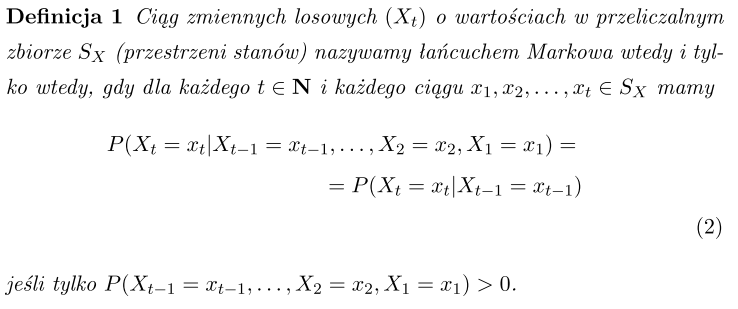
\includegraphics[width=0.80\linewidth]{definicja.PNG}
	\label{definicja}
\end{figure}

Warunek w powyższej definicji określa cały charakter łańcuchów Markowa, czyli, że ewolucja procesu zależy tylko i wyłącznie od bieżącego stanu. Zatem na charakter zmiennej $X_t$ w zadanej chwili $t$ ma wpływ wartość procesu w chwili $t - 1$. Taki łańcuch nazywamy łańcuchem Markowa rzędu pierwszego, czyli jego stan zależy tylko od stanu poprzedniego. Istnieją także rzędy \textit{x}, mówiące, że stan zależy od \textit{x}-stanów poprzednich.

W wypadku, gdy prawdopodobieństwa przejścia między stanami nie zależą od momentu, w którym rozpatrywany jest proces, wtedy łańcuch określić można mianem jednorodnego w czasie. Prawdopodobieństwo takie oznacza się jako $p_{ij}$. Macierz kwadratowa $P=[p_{ij}]$ jednorodnego łańcucha Markowa określa się jako macierz przejść.

\subsubsection{Definicja ukrytego modelu Markowa}

Dla rozważań w tym rozdziale, niech:

\begin{description}
  \item[T] = długość obserwowanej sekwencji
  \item[N] = liczba stanów w modelu
  \item[M] = liczba obserwacji
\end{description}

Mając na uwadze, że ukryty model Markowa jest szczególnym przypadkiem łańcuchu Markowa, możemy teraz opisać ten układ. Przejścia między stanami opisane niech będą przy pomocy kwadratowej macierzy prawdopodobieństw $A=[a_{ij}]$, gdzie element $a_{ij}$ jest to prawdopodobieństwo przejścia od stanu $i$ do stanu $j$ w następnej chwili czasowej.

$$ a_{ij}=Pr(x_{t}=j\,|\,x_{t-1}=i) \quad dla \quad 1 \leq i,j \leq N $$

Spełniona jest równość:

$$ \sum_{j=1}^{N} a_{ij} = 1 $$

\newpage

Kolejną składową systemu jest macierz $\Pi$ zawierająca prawdopodobieństwa wystąpienia \textbf{i}-tego stanu na początku sekwencji stanów.

$$ \Pi_{i} = Pr(x_{0}=1) $$

Znając obie macierze A oraz $\Pi$ można obliczyć prawdopodobieństwo wygenerowania przez system sekwencji stanów $X=(x_{0},x_{1}, \dots, x_{T})$.

$$ Pr(x\,|\,A,\Pi) = \Pi_{x_{0}}a_{x_{0}x_{1}}a_{x_{1}x_{2}} \dots x_{x_{T-1}x_{T}} $$

Tak opisana została warstwa ukryta. Model ten posiada jednakże jeszcze drugą warstwę, określaną mianami warstwy ukrytej, obserwowanej, bądź emisji. Każdemu ze stanów ukrytych przypada pewne prawdopodobieństwo $b$, mówiące, że w trakcie przebywania w nim, wygenerowana zostanie obserwacja $O_{t}$.

$$ B=\{b_{i}(O_{t})\}_{i=1}^{N} $$

Posiadając te wszystkie informacje można określić ukryty model Markowa jako $\lambda$:

$$ \lambda = (\Pi,A,B) $$

Teraz można obliczyć prawdopodobieństwo wygenerowania sekwencji obserwacji $O$ przez system $\lambda$:

$$ Pr(O\,|\,\Pi,A,B) = \sum_{x}P(O,x\,|\,\Pi,A,B) = \sum_{x}\Pi_{x_{0}}\prod_{t=1}^{T}a_{x_{t-1}x_{t}}b_{x_{t}}(O_{t}) $$

Ukryty model Markowa najprościej jest zobrazować przy pomocy poniższego schematu, zwanego grafem \textit{Trellisa}, gdyż ukazuje zmienność procesu wraz z czasem. Linią kropkowaną oddzielono to co widoczne jest przez obserwatora od warstwy ukrytej. Strzałki między węzłami mówią o bezpośredniej zależności stochastycznej, zaś brak strzałki oznacza niezależność losową.

\begin{figure}[h!]
	\centering
	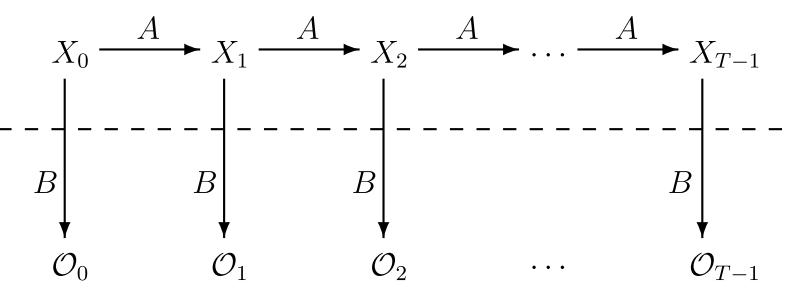
\includegraphics[width=0.70\linewidth]{markov-model.PNG}
	\label{markov-model}
	\caption{Ukryty model Markowa}
\end{figure}

Gdzie:

\begin{description}
  \item[X] = ($X_0, X_1, ..., X_{T-1}$) ukryte stany
  \item[O] = ($O_0, O_1, ..., O_{T-1}$) sekwencja obserwacji
  \item[A] = macierz prawdopodobieństw przejść między stanami
  \item[B] = macierz prawdopodobieństw wystąpienia obserwacji (emisji)
\end{description}
